%pictures and spectra
%tables and graphs
%statements of the result

%%% three subfigures next to each others
% \begin{figure*}
%     \centering
% \begin{subfigure}{.3\textwidth}
%     \centering
%     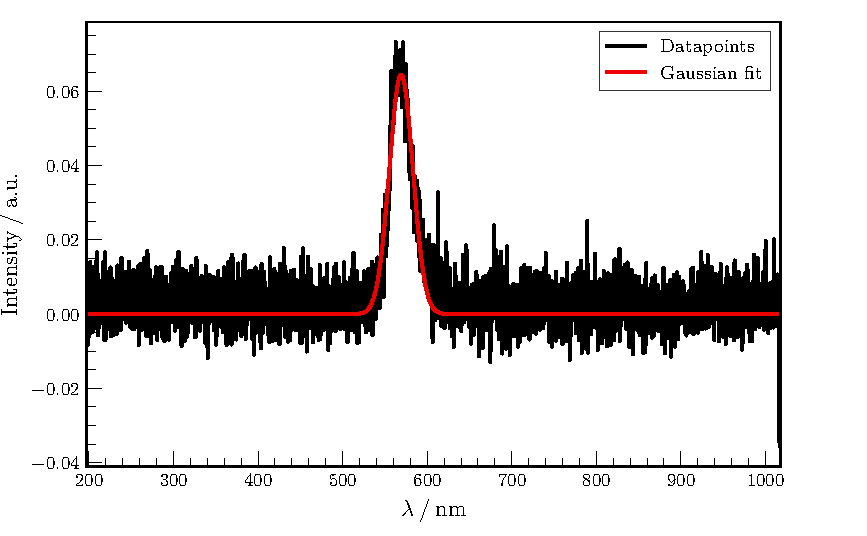
\includegraphics[width=\textwidth]{plots/LED-Green.pdf}
%     \caption{Green LED lightsourse}
%     \label{fig:LEDG}
% \end{subfigure}
% \begin{subfigure}{.3\textwidth}
%     \centering
%     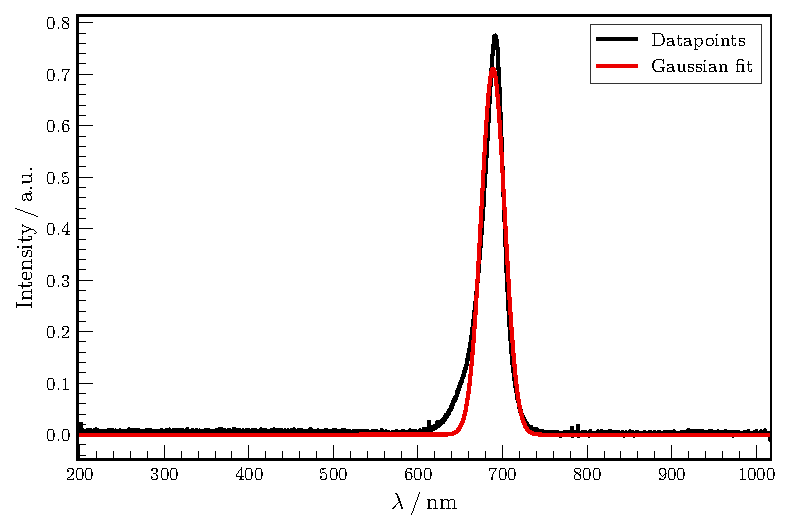
\includegraphics[width=\textwidth]{plots/LED-Red.pdf}
%     \caption{Red LED lightsourse}
%     \label{fig:LEDR}
% \end{subfigure}
% \begin{subfigure}{.3\textwidth}
%     \centering
%     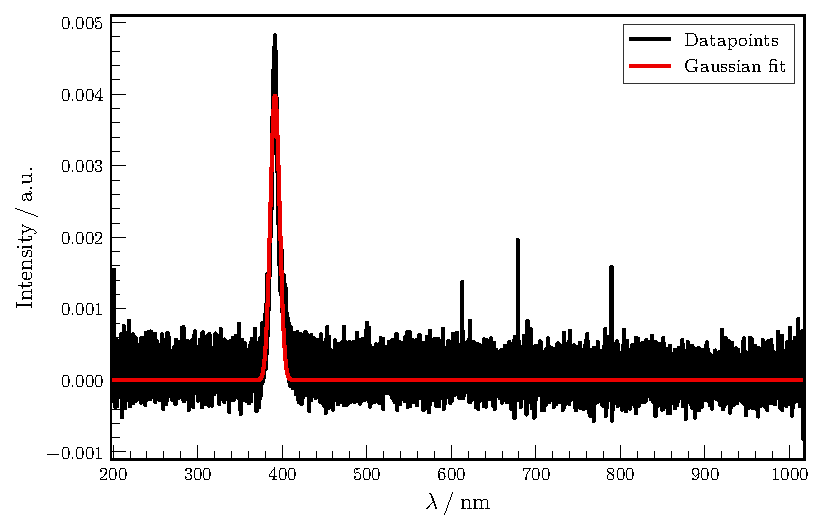
\includegraphics[width=\textwidth]{plots/LED-UV.pdf}
%   \caption{UV LED lightsourse}
%     \label{fig:LEDUV}
% \end{subfigure}
% \caption{Spectral measurement of different LED lightsourse. A Gaussian fit is implemented around the emmision peak.}
% \end{figure*}

%%one figure inside the collums
% \begin{figure}
%     \captionsetup{width=0.9\linewidth}
%     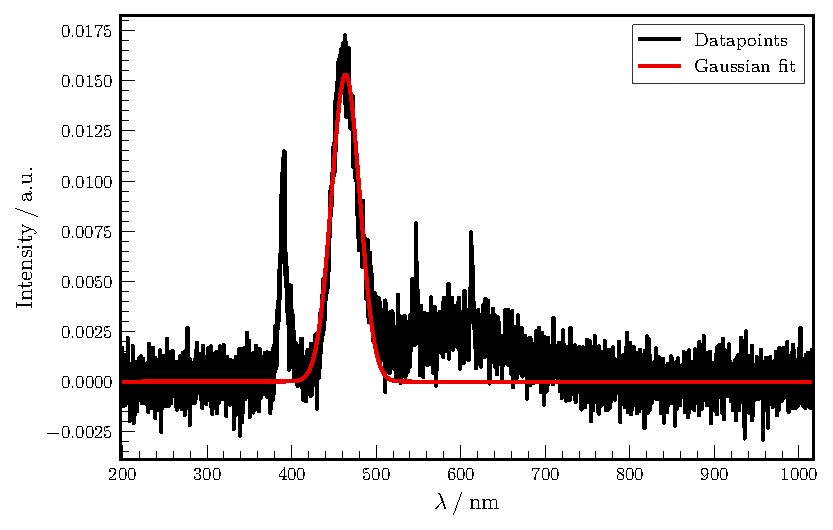
\includegraphics[width=0.5\textwidth]{plots/Samp_A_D.pdf}
%   \caption{Spectral measurement of sample A, excited by a UV-LED lightsource. A Gaussian fit of the peak contributed by luminescense is implemented.}
%     \label{fig:Samp_A_D}
% \end{figure}

\section{Results}
\label{sec:Results}

Figure \ref{fig:comparison} shows the normalized resistance of the germanium, copper and nickel samples in a temperature range from $\SI{114.286}{\kelvin}$ up to $\SI{451.038}{\kelvin}$.
The normalizing value is the sample specific resitance at $\SI{0}{\celsius}$.

\begin{figure*}
    \captionsetup{width=0.9\linewidth}
    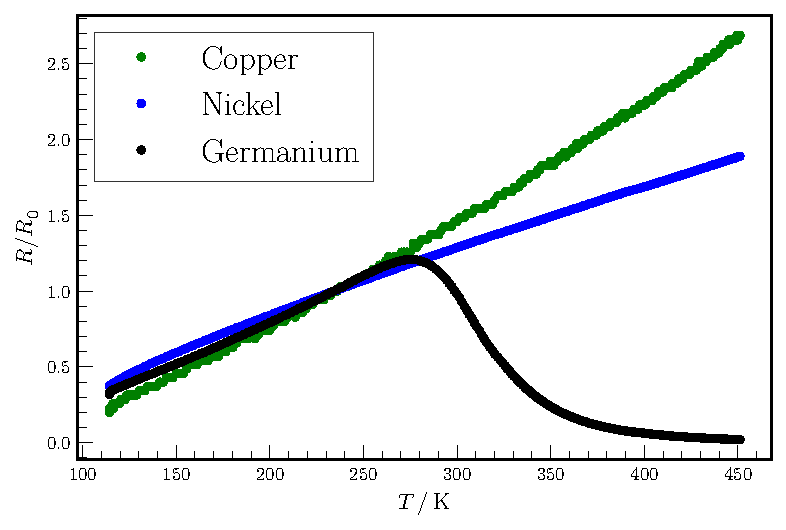
\includegraphics[width=0.7\textwidth]{plots/compare.pdf}
  \caption{Resistance measurement of germanium, copper and nickel, displayed in a nomalized plot based on the resistance at $\SI{0}{\celsius}$.}
    \label{fig:comparison}
\end{figure*}

In figure \ref{fig:metalic-fit} a linear regression in the from
\begin{equation}
    R(T) = R_0 (1+\beta T)
\end{equation}
has been done and added in the plots. 
As this linear relation describes the metallic behavior, therefore for the semiconductor only the low temperature data up to a temperature of $\SI{260}{\kelvin}$ have been taken into acount.

%% three subfigures next to each others
\begin{figure*}
    \centering
\begin{subfigure}{.3\textwidth}
    \centering
    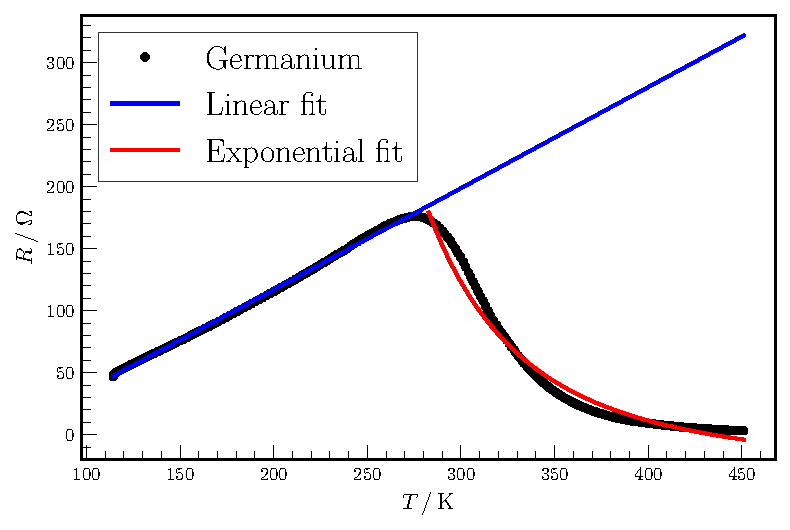
\includegraphics[width=\textwidth]{plots/R1.pdf}
    \caption{Germanium}
    \label{fig:Ge}
\end{subfigure}
\begin{subfigure}{.3\textwidth}
    \centering
    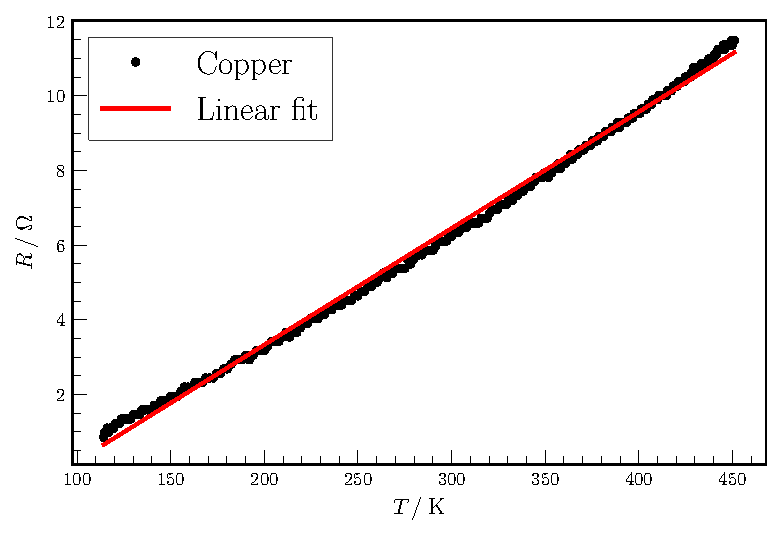
\includegraphics[width=\textwidth]{plots/R2.pdf}
    \caption{Copper}
    \label{fig:Cu}
\end{subfigure}
\begin{subfigure}{.3\textwidth}
    \centering
    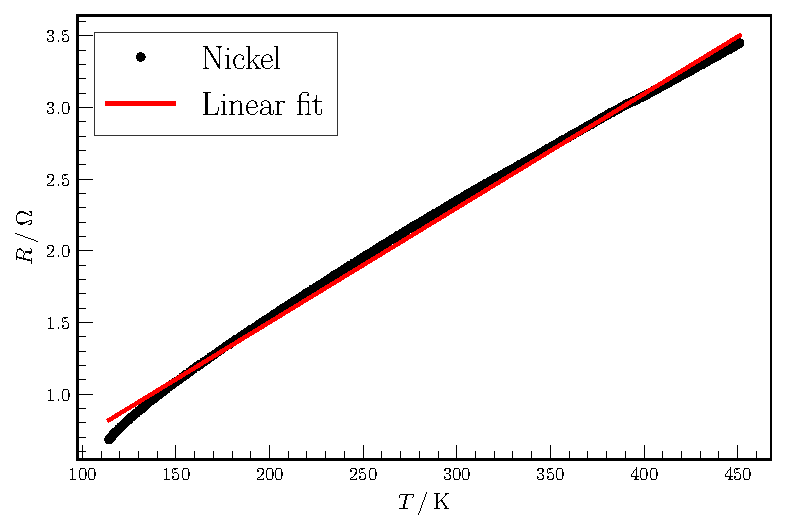
\includegraphics[width=\textwidth]{plots/R3.pdf}
  \caption{Nickel}
    \label{fig:Ni}
\end{subfigure}
\caption{Temperature-dependent resistance of three samples, including a linear regression based (In the case of germanium only the datapoints with a temperature lower then $\SI{260}{\kelvin}$ have been evaluated.)}
\label{fig:metalic-fit}
\end{figure*}

The resulting fitting parameters $\beta$ are
\begin{align*}
    \beta(Ge) &= \SI{8.15 \pm 0.04 e-1}{\per\kelvin} \\
    \beta(Cu) &= \SI{3.118 \pm 0.001 e-2}{\per\kelvin} \\
    \beta(Ni) &= \SI{7.966 \pm 0.001 e-3}{\per\kelvin} \\
\end{align*}